\begin{figure}[h]
	\centering

	\begin{tabular}{c | c c c c}
		% Outline:
		%   s\g |  250k | 500k | 750k | 1mm
		%	0.25
		%   0.50
		%   1.00
		%   1.50
		$s$ \textbf{\textbackslash} game & 250,000 & 500,000 & 750,000 & 1,000,000 \\
		\hline
		\\
		0.25 & % a & b & c & d
			\parbox[c]{5em}{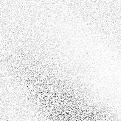
\includegraphics[width=\stratgraphwidthsmall]{images/findings/experiments/learning_rate/lr_025_250.png}} & % 250
			\parbox[c]{5em}{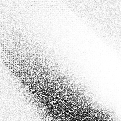
\includegraphics[width=\stratgraphwidthsmall]{images/findings/experiments/learning_rate/lr_025_500.png}} & % 500
			\parbox[c]{5em}{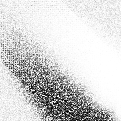
\includegraphics[width=\stratgraphwidthsmall]{images/findings/experiments/learning_rate/lr_025_750.png}} & % 750
			\parbox[c]{5em}{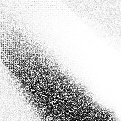
\includegraphics[width=\stratgraphwidthsmall]{images/findings/experiments/learning_rate/lr_025_1mm.png}} \\ % 1mm
		\\
		0.50 & 
			\parbox[c]{5em}{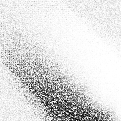
\includegraphics[width=\stratgraphwidthsmall]{images/findings/experiments/learning_rate/lr_050_250.png}} & % 250
			\parbox[c]{5em}{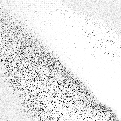
\includegraphics[width=\stratgraphwidthsmall]{images/findings/experiments/learning_rate/lr_050_500.png}} & % 500
			\parbox[c]{5em}{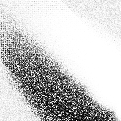
\includegraphics[width=\stratgraphwidthsmall]{images/findings/experiments/learning_rate/lr_050_750.png}} & % 750
			\parbox[c]{5em}{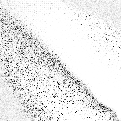
\includegraphics[width=\stratgraphwidthsmall]{images/findings/experiments/learning_rate/lr_050_1mm.png}} \\ % 1mm
		\\
		0.75 & 
			\parbox[c]{5em}{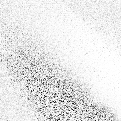
\includegraphics[width=\stratgraphwidthsmall]{images/findings/experiments/learning_rate/lr_075_250.png}} & % 250
			\parbox[c]{5em}{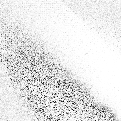
\includegraphics[width=\stratgraphwidthsmall]{images/findings/experiments/learning_rate/lr_075_500.png}} & % 500
			\parbox[c]{5em}{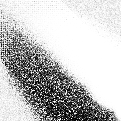
\includegraphics[width=\stratgraphwidthsmall]{images/findings/experiments/learning_rate/lr_075_750.png}} & % 750
			\parbox[c]{5em}{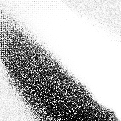
\includegraphics[width=\stratgraphwidthsmall]{images/findings/experiments/learning_rate/lr_075_1mm.png}} \\ % 1mm
		\\
		1.50 & 
			\parbox[c]{5em}{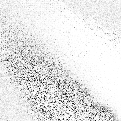
\includegraphics[width=\stratgraphwidthsmall]{images/findings/experiments/learning_rate/lr_150_250.png}} & % 250
			\parbox[c]{5em}{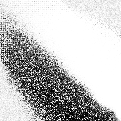
\includegraphics[width=\stratgraphwidthsmall]{images/findings/experiments/learning_rate/lr_150_500.png}} & % 500
			\parbox[c]{5em}{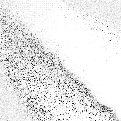
\includegraphics[width=\stratgraphwidthsmall]{images/findings/experiments/learning_rate/lr_150_750.png}} & % 750
			\parbox[c]{5em}{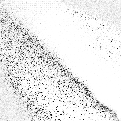
\includegraphics[width=\stratgraphwidthsmall]{images/findings/experiments/learning_rate/lr_150_1mm.png}} \\ % 1mm
	\end{tabular}

\caption{
	Comparison of different scaling factors ($s$),
	learning the \handmaxavg\ strategy
	when playing as the pone
	over the course of one million games.
	For comparison, $s = 10.0$ and $s = 2.0$ for Rounds 1 and 2, respectively
	(see Figures~\ref{fig_r1-flip} and~\ref{fig:r2-flip-loser}).
	}
\label{fig:expts-lr-comp}
\end{figure}
